\documentclass[11pt,a4paper]{article}

\usepackage[utf8]{inputenc}
\usepackage[T1]{fontenc}
\usepackage[brazil]{babel}
\usepackage[a4paper, margin=2.2cm]{geometry}
\usepackage{xcolor}
\usepackage{listings}
\usepackage{tcolorbox}
\usepackage{hyperref}
\usepackage{fancyhdr}
\usepackage{titling}
\usepackage{enumitem}
\usepackage{graphicx}
\usepackage{caption}
\tcbuselibrary{skins, breakable, listings}

% Cores
\definecolor{termbg}{HTML}{1E1E1E}
\definecolor{termfg}{HTML}{D4D4D4}
\definecolor{codebg}{HTML}{F7F7F7}
\definecolor{codekw}{HTML}{0000FF}
\definecolor{codestr}{HTML}{A31515}
\definecolor{codecomm}{HTML}{008000}
\definecolor{titleblue}{HTML}{1F4E79}

% Estilo do codigo C
\lstdefinestyle{cstyle}{
  language=C,
  basicstyle=\ttfamily\small,
  keywordstyle=\color{codekw}\bfseries,
  stringstyle=\color{codestr},
  commentstyle=\color{codecomm}\itshape,
  numbers=left,
  numberstyle=\tiny\color{gray},
  numbersep=8pt,
  backgroundcolor=\color{codebg},
  frame=single,
  rulecolor=\color{black!30},
  showstringspaces=false,
  breaklines=true,
  tabsize=4,
  captionpos=b,
  inputencoding=utf8,
  extendedchars=true,
  literate={á}{{\'a}}1 {â}{{\^a}}1 {ã}{{\~a}}1 {à}{{\`a}}1
           {é}{{\'e}}1 {ê}{{\^e}}1 {í}{{\'i}}1
           {ó}{{\'o}}1 {ô}{{\^o}}1 {õ}{{\~o}}1
           {ú}{{\'u}}1 {ç}{{\c{c}}}1
           {Á}{{\'A}}1 {É}{{\'E}}1 {Í}{{\'I}}1 {Ó}{{\'O}}1 {Ú}{{\'U}}1
}

% Caixa para a captura de tela
\newtcolorbox{screenshot}[1][]{
  enhanced,
  colback=black!90,
  colframe=black!70,
  arc=3pt,
  boxrule=0.6pt,
  before skip=8pt, after skip=8pt,
  left=4pt, right=4pt, top=6pt, bottom=6pt,
  attach boxed title to top left={xshift=12pt, yshift=-9pt},
  boxed title style={
    colback=black!85, colframe=black!70,
    arc=2pt, boxrule=0.4pt, size=fbox
  },
  coltitle=white,
  fonttitle=\sffamily\footnotesize\bfseries,
  title={\textcolor{red!80!white}{$\bullet$}\,\textcolor{yellow!80!white}{$\bullet$}\,\textcolor{green!70!white}{$\bullet$}\quad bash},
  breakable,
  #1
}

% Cabecalho
\pagestyle{fancy}
\fancyhf{}
\fancyhead[L]{\small Sistemas Operacionais}
\fancyhead[R]{\small Vinicius Guerra}
\fancyfoot[C]{\thepage}
\renewcommand{\headrulewidth}{0.4pt}

\title{
  \vspace{-1.5cm}
  {\Large \textcolor{titleblue}{\textbf{Atividade: Condição de Disputa}}}\\[2pt]
  \large Aula 03, Interação entre Tarefas (Parte II)
}
\author{
  Vinicius Guerra \\
  IFSC, Campus São José \\
  Eng. de Telecomunicações
}
\date{Maio de 2026}

\begin{document}
\maketitle
\thispagestyle{fancy}

\section*{Enunciado}
O slide final da aula pede para aplicar três algoritmos de exclusão mútua
ao código de depósito bancário concorrente. O código tem uma condição
de disputa porque a leitura e a escrita do \texttt{saldo} acontecem em
momentos diferentes:
\begin{enumerate}[noitemsep, topsep=2pt]
  \item Alternância de Uso (\textit{strict turn-taking})
  \item Algoritmo de Peterson (1981)
  \item TSL, \textit{Test-and-Set Lock} (operação atômica)
\end{enumerate}

\noindent
Em todos os testes uso \texttt{saldo=100}, \texttt{v1=50} e \texttt{v2=30}.
O resultado correto é 180.

\vspace{4pt}
\hrule
\vspace{6pt}

% =====================================================================
\section{Demonstração da Condição de Disputa}

O código original não tem nenhum mecanismo de exclusão mútua. As três
operações (ler, somar, escrever) das duas \textit{threads} se intercalam
e um dos depósitos acaba sendo perdido. O \texttt{usleep(100)} entre a
leitura e a escrita aumenta a chance de troca de contexto e ajuda a
expor o problema.

\lstinputlisting[style=cstyle, caption={\texttt{0\_problema.c}: código original com condição de disputa}]{codigos/0_problema.c}

\subsection*{Captura de tela}

\begin{screenshot}
\centering
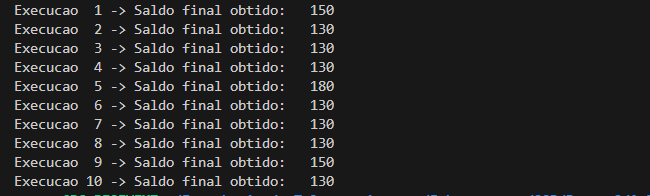
\includegraphics[width=0.92\linewidth]{imgs/image1.png}
\end{screenshot}

\begin{center}
\small \textit{Figura 1: 10 execuções do código original sem proteção.}
\end{center}

O resultado é não-determinístico. Na maior parte das execuções o saldo
final é 130 ou 150, e raramente 180 (quando o escalonador, por sorte, não
intercala as operações). Quando t1 e t2 leem \texttt{saldo=100} antes de
qualquer escrita, o último a gravar sobrescreve o depósito do outro e o
sistema perde 50 ou 30 reais.

\newpage
% =====================================================================
\section{Solução 1: Alternância de Uso}

Uma variável global \texttt{turn} indica de quem é a vez. A tarefa só
entra na seção crítica quando \texttt{turn == task}, e ao sair passa o
turno para a próxima.

\lstinputlisting[style=cstyle, caption={\texttt{1\_alternancia.c}}]{codigos/1_alternancia.c}

\subsection*{Captura de tela}

\begin{screenshot}
\centering
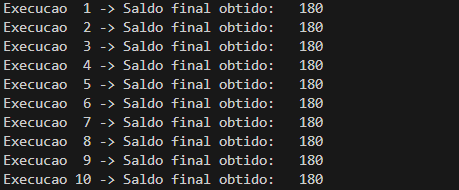
\includegraphics[width=0.92\linewidth]{imgs/image2.png}
\end{screenshot}

\begin{center}
\small \textit{Figura 2: 10 execuções com alternância de uso. Saldo final sempre 180.}
\end{center}

A solução resolve a disputa, mas cria uma dependência rígida entre as
tarefas. Se a tarefa 0 não quiser entrar, a tarefa 1 fica esperando o
turno indefinidamente. Por isso ela falha no critério de independência.

\newpage
% =====================================================================
\section{Solução 2: Algoritmo de Peterson}

Cada tarefa sinaliza interesse (\texttt{wants[task]=1}) e cede o turno
para a outra (\texttt{turn=other}). O \texttt{while} só bloqueia se a
outra também quer entrar e for a vez dela.

\lstinputlisting[style=cstyle, caption={\texttt{2\_peterson.c}}]{codigos/2_peterson.c}

\subsection*{Captura de tela}

\begin{screenshot}
\centering
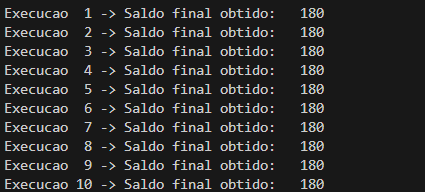
\includegraphics[width=0.92\linewidth]{imgs/image3.png}
\end{screenshot}

\begin{center}
\small \textit{Figura 3: 10 execuções com Peterson. Saldo final sempre 180.}
\end{center}

Aqui o resultado também é correto e a independência fica preservada: se
só uma tarefa quer entrar, ela entra imediatamente. As limitações são
que o algoritmo só funciona para duas tarefas e mantém espera ocupada.
Precisei usar \texttt{\_\_sync\_synchronize()} para impedir que o
compilador e a CPU reordenassem as escritas em \texttt{wants} e \texttt{turn},
o que poderia quebrar a lógica do algoritmo.

\newpage
% =====================================================================
\section{Solução 3: TSL (Test-and-Set Lock)}

A instrução TSL lê o valor antigo e escreve 1 num único passo atômico.
No código uso a built-in \texttt{\_\_sync\_lock\_test\_and\_set} do GCC,
que gera a instrução equivalente no x86 (\texttt{XCHG} ou \texttt{LOCK CMPXCHG}).
Funciona para qualquer número de tarefas e em multiprocessadores.

\lstinputlisting[style=cstyle, caption={\texttt{3\_tsl.c}}]{codigos/3_tsl.c}

\subsection*{Captura de tela}

\begin{screenshot}
\centering
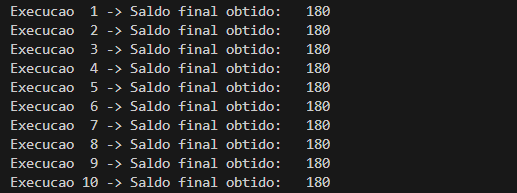
\includegraphics[width=0.92\linewidth]{imgs/image4.png}
\end{screenshot}

\begin{center}
\small \textit{Figura 4: 10 execuções com TSL. Saldo final sempre 180.}
\end{center}

Resolve a disputa, vale para $N$ tarefas e roda em sistemas com vários
núcleos. O único ponto fraco é a espera ocupada. É a base usada pelos
mutexes reais do Linux (\texttt{pthread\_mutex\_t}).

\section*{Conclusão}

Sem nenhum mecanismo de proteção, três operações simples (ler, somar e
escrever) sobre uma variável compartilhada produzem resultados
imprevisíveis: nas 10 execuções tive 130, 150 e ocasionalmente 180.
As três soluções vistas em aula corrigem o problema e o saldo final
passa a ser sempre 180.

Cada uma tem limitações próprias. A alternância é rígida, o Peterson só
serve para duas tarefas, e todas usam espera ocupada. Por isso, na
prática usa-se mecanismos mais robustos como mutexes e semáforos.

\end{document}
